\chapter{Source code structure}

\section{Application server}

The application server project tree follows a distributed MVC approach combined with Clean Architecture principles.
This structure ensures a clear separation of concerns, maintaining independent layers for application logic, domain rules, and infrastructure. By organizing the code in this way, we improve maintainability, scalability, and testability across the system.

\begin{figure}[H]
    \centering
    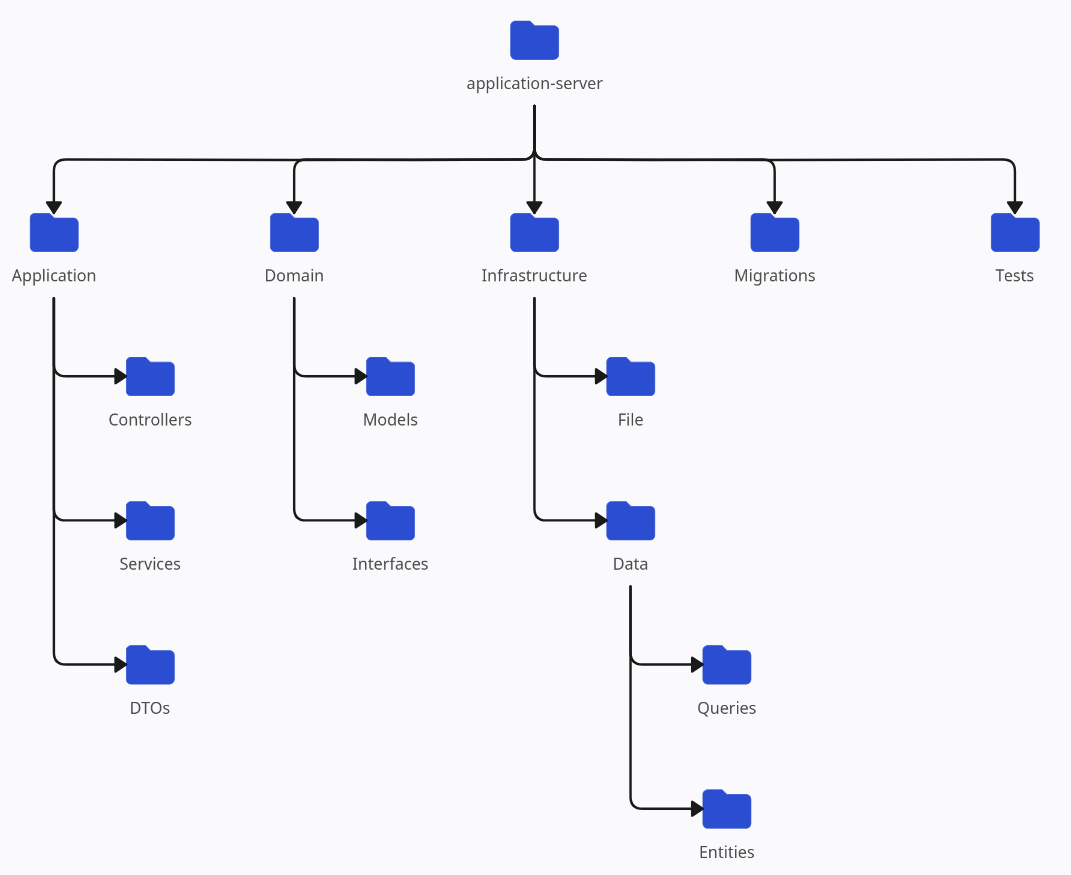
\includegraphics[width=0.8\linewidth]{../assets/folder-tree/application-server.png}
\end{figure}

\section{Web server}

The web server is organized with a modular structure to ensure scalability and maintainability.
There are two main folders, one containing the core application logic, and the other holding static assets, supporting the separation of UI components and resources from the application’s core functionality.

\begin{figure}[H]
    \centering
    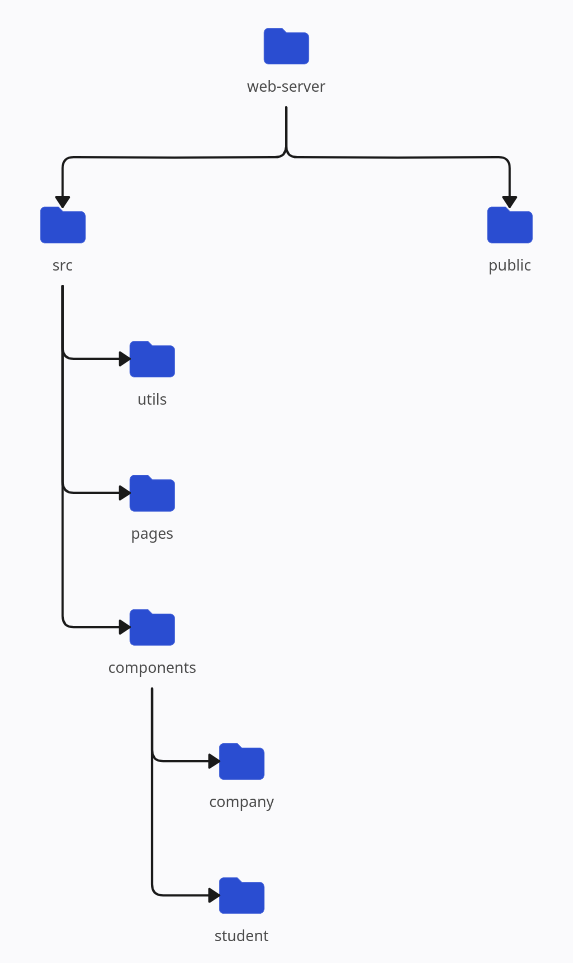
\includegraphics[width=0.5\linewidth]{../assets/folder-tree/web-server.png}
\end{figure}

